\section{Clustering par partionement}
Nous avons réalisé le clustering par partitionnement à l'aide du composant hierarchical Clustering avec la configuration Linkage type : COMPLETE. Pour observer les résultats nous avons utilisé le composant Scatter Matrix.

\subsection{Santé}
Nous avions choisi de faire 3 clusters (cf section précédente), dont la répartitions des pays se fait comme suit : 

\begin{figure}[H]
	\begin{center}
		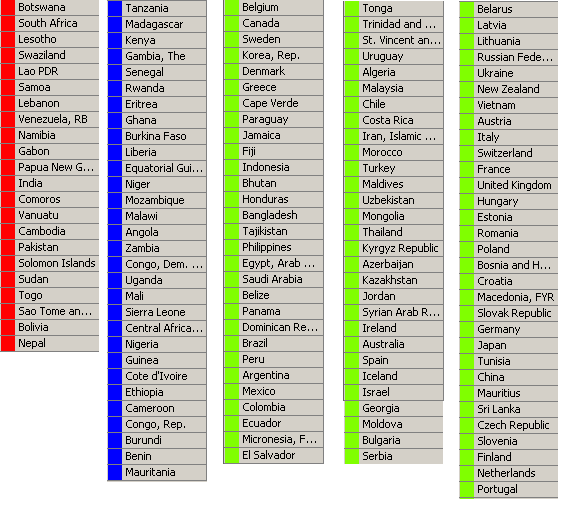
\includegraphics[scale=0.5]{Image/TableViewSanteNoMissing2}
		\caption{Liste des pays par clusters sur les critères de santé avec le jeu \jeuc}
	\end{center}
\end{figure}


Nous obtenons les résultats suivants : 

\begin{figure}[H]
	\begin{center}
		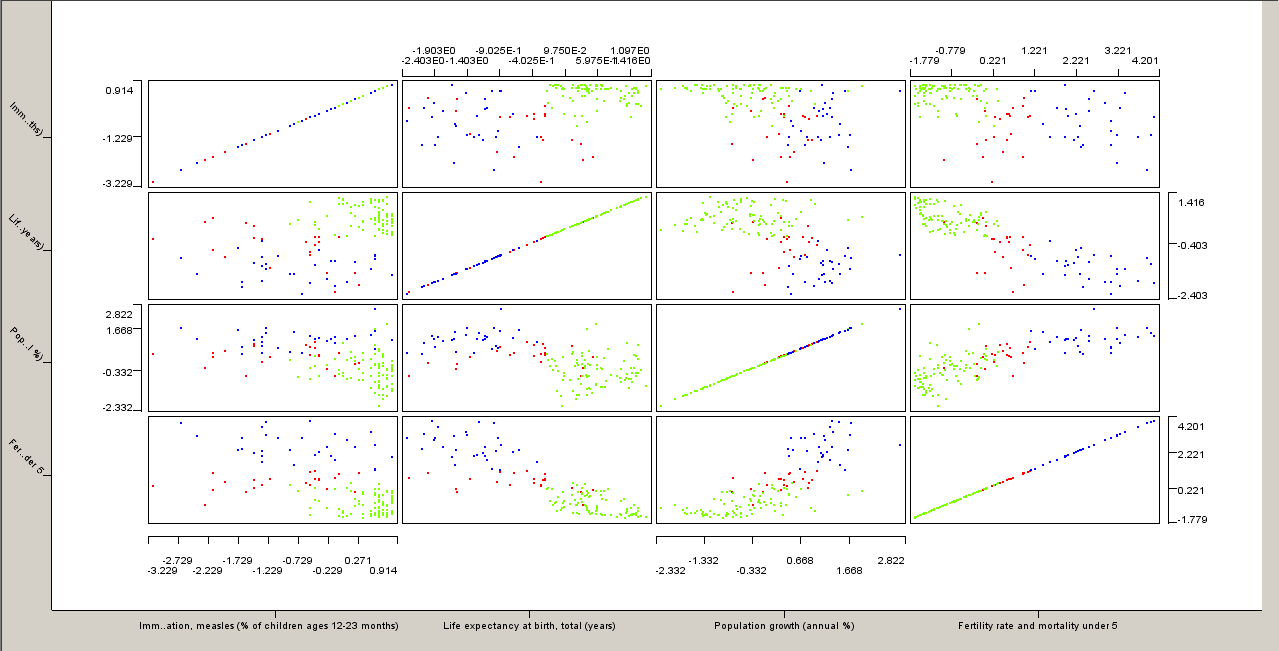
\includegraphics[scale=0.5]{Image/ScatterMatrixSanteNoMissing2}
		\caption{Scatter Matrix des attributs de l'indicateur Santé \jeuc}
	\end{center}
\end{figure}

\paragraph{Analyse}
TODO : si j'ai bien compris c'est plutot cool :)

\subsection{Économie}
Au vu des distances obtenues dans la section précédente, nous obtenons 4 clusters.

\begin{figure}[H]
	\begin{center}
		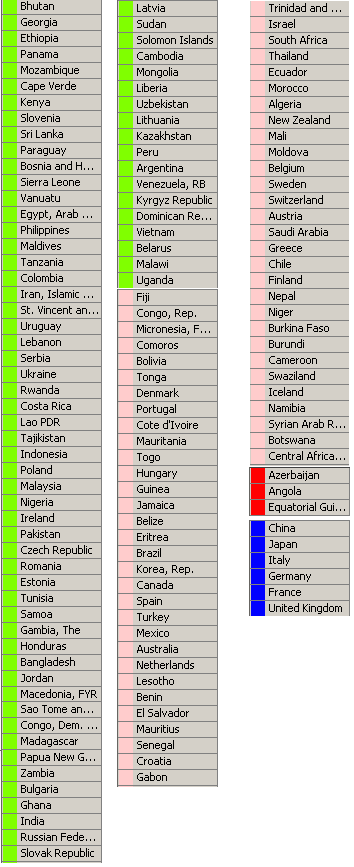
\includegraphics[scale=0.5]{Image/TableViewPolitiqueNoMissing2}
		\caption{Liste des pays par clusters sur les critères économiques avec le jeu \jeuc}
	\end{center}
\end{figure}


Nous obtenons les résultats suivants : 

\begin{figure}[H]
	\begin{center}
		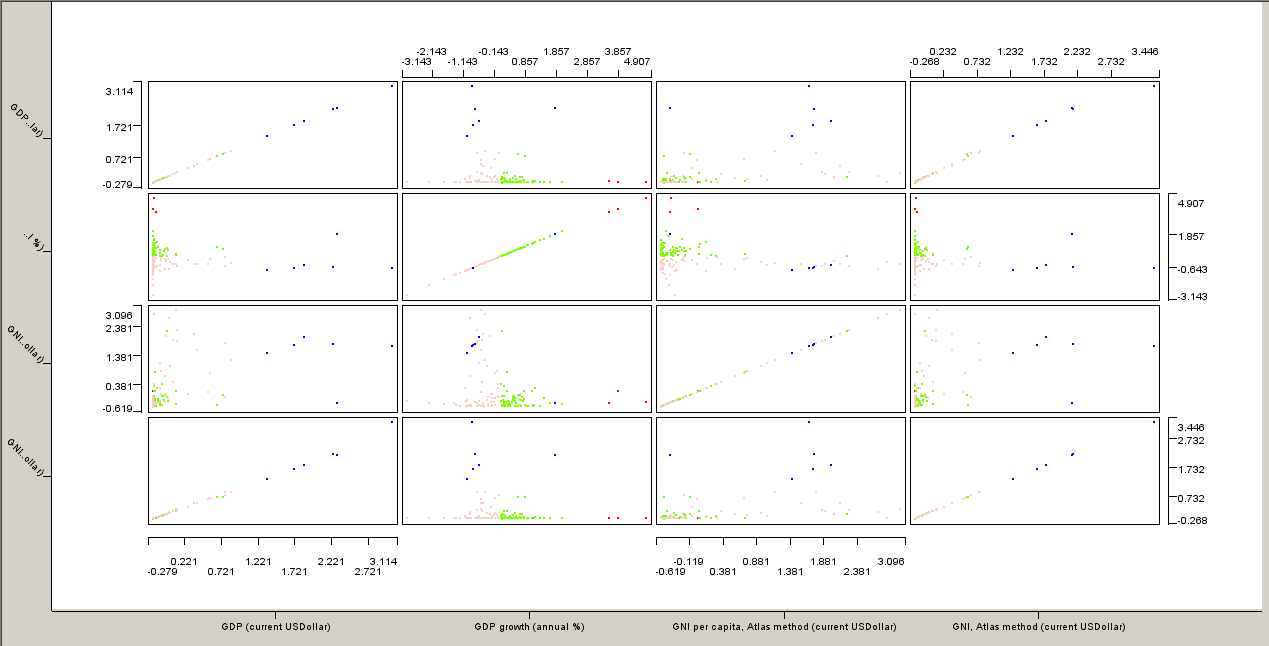
\includegraphics[scale=0.5]{Image/ScatterMatrixPolitiqueNoMissing2}
		\caption{Scatter Matrix des attributs de l'indicateur de politique économique \jeuc}
	\end{center}
\end{figure}

\paragraph{Analyse}
TODO : si j'ai bien compris c'est pas clair :)



